% !TeX root = ../latex-curto.tex
% !TeX encoding = utf8

\section{TikZ}

\begin{frame}
  \frametitle{\Tikz}
  
  \begin{itemize}
  \item O \Tikz\ é uma linguagem que gera figuras, a partir de uma
    descrição da mesma em termos de linhas, formas e texto.
  \item gráficos são vetoriais e de alta qualidade
  \item já são parte do documento \tikz \draw[color=blue,thick] (0,0)
    circle (.7ex); sendo \tikz \draw[rotate=20,purple,thick] (0,0) rectangle
    (1ex,.6ex); fáceis 
    \tikz \draw[thick,green!50!black] (0,0) -- (1ex,0) -- (60:1ex) --cycle;
    de misturar.
  \end{itemize}


 
\end{frame}

\begin{frame}
  \frametitle{Figuras com \Tikz}

  \begin{itemize}
  \item Usar pacote \green{\texttt{tikz}} no preâmbulo
  \item Usar ambiente \blue{\texttt{tikzpicture}}
  \item Dentro do ambiente, usar \brown{comandos} como\\
    \purple{\texttt{\bs draw}} --- para traçar linhas\\
    \purple{\texttt{\bs fill}} --- para áreas preenchidas\\
    \purple{\texttt{\bs node}} --- para escrever texto\\
    que \green{terminam com ponto-e-vírgula ``\texttt{;}''}
  \item tem \green{parâmetros opcionais} para alterar estilos
    de linha e preenchimento

  \end{itemize}
\end{frame}

\begin{frame}
  \frametitle{Exemplo}

\begin{multicols}{2}
\begin{code*}\footnotesize
\string\begin\ac{}tikzpicture\fc{}\\
\string\draw[blue]\ (0,1)\ --\ (1,0);\\
\string\end\ac{}tikzpicture\fc{}
\end{code*}

\begin{tikzpicture}
\draw[->,blue]  (0,1) -- (1,0);
\end{tikzpicture}
\end{multicols}
  
\end{frame}

\section{Coordenadas e marcas aos pontos}

\begin{frame}
  \frametitle{Pontos}

  \begin{block}{Pontos}
    Dois valores entre parênteses.
  \end{block}
\bigskip

  Podem ser em \green{coordenadas}
  \begin{description}
  \item[cartesianas] valores $(x,y)$ separados por \green{vírgula ``\texttt{,}''} --- \texttt{(0,1)}
  \item[polares] valores $(\theta:r)$ separados por \green{2-pontos
    ``\texttt{:}''} --- \texttt{(30:1)}
  \end{description}
\end{frame}

\begin{frame}
  \frametitle{Coordenadas em valor absoluto ou relativo}

  \begin{block}{Tipos de coordanadas}
    \begin{description}
    \item[absoluto] Determina o ponto\\
      \blue{\texttt{(1,0)}} --- ponto de coordenadas $(1,0)$.
    \item[relativo] Adiciona à posição atual: comece ponto com
      \green{\texttt{++}}
      \blue{\texttt{++(1,0)}} --- se o ponto anterior era $(2,2)$, vai
      para o ponto $(3,2)$.
    
    \item[cruzamento] Ponto definido pelo cruzamento da \blue{vertical horizontal por um ponto A} e pela \green{horizontal por outro ponto B}:\\
      \texttt{\green{(}{\blue{\textit{A}} \purple{|-} \blue{\textit{B}}\green{)}}}
    % \item[relativo sem atualização] Adiciona à posição atual\\
    %   mas \red{não atualiza posição}:\\ comece ponto com \green{\texttt{+}}.

    %   Exemplo: \blue{\texttt{+(1,0)}} --- se o ponto anterior era
    %   $(2,2)$, denota o ponto $(3,2)$, mas ponto atual fica em
    %   $(2,2)$.
    \end{description}
  \end{block}

\end{frame}

\begin{frame}

  \frametitle{Exemplo}

\centering

  \begin{tikzpicture}[scale=4,>=stealth]
    \draw[gray,dotted] (50:1) coordinate (A) -- node[midway,above left] {$1$}
    (0,0) coordinate (O) -- (1.5,0);
    \draw[thin,->,gray] (0:.2) arc (0:50:.2);
    \node[gray] at (20:.3) {$50^{\circ}$};
    \fill (0,0) circle (.3pt) (A) circle (.3pt)
          ++(-30:.5) coordinate (B) circle (.3pt)
          (O |- A) coordinate (OA) circle (.3pt);

    \draw[gray,dotted] (A) +(.3,0) -- +(-1.3,0) (0,-.2)--(0,.9); 
    \draw[gray,dotted] (A) -- node[midway,below left=-1mm] {\scriptsize$0.5$} (B) ;
    \begin{scope}[shift={(A)}]\scriptsize
      \draw[thin,->,gray] (0:.2) arc (0:-30:.2);
      \node[gray] at (-12:.3) {$-30^{\circ}$};
      
    \end{scope}


    \node[left] at (O) {\blue{\texttt{(0,0)}}};
    \node[above] at (A) {\green{\texttt{(50:1)}}};
    \node[above left] at (OA) {\purple{\texttt{(0,0 |- 50:1)}}};
    \node[right] at (B) {\red{\texttt{(50:1) ++(-30:.5)}}};
  \end{tikzpicture}
\end{frame}


\begin{frame}
  \frametitle{Comando \texttt{coordinate}}

  \begin{block}{\texttt{coordinate}}
  Após escrever um ponto, adicionar\\
    \mbox{}\hfill\purple{\texttt{coordinate (\texttt{nome})}}\hfill\mbox{} \\
    para nomeá-lo para usar em comandos futuros.
  \end{block}

  \begin{exampleblock}{}\small
    \texttt{\string\begin\ac{}tikzpicture\fc{}\\
    \ \ \string\draw[->]\ \purple{(0,0)\ coordinate\ (A)}\ --
    \blue{(30:1)\ coordinate\ (B)};\\
    \ \ \string\draw[thick,\ dotted]\ \purple{(A)}\ --\ (1,0)\ --\ \blue{(B)};\\
    \string\end\ac{}tikzpicture\fc{}\\}

\centering
    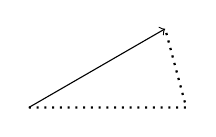
\begin{tikzpicture}[scale=2]
      \draw[->] (0,0) coordinate (A) -- (30:1) coordinate (B);
      \draw[thick, dotted] (A) -- (1,0) -- (B);
    \end{tikzpicture}

  \end{exampleblock}

\end{frame}

\section{Caminhos}

\begin{frame}
  \frametitle{Tipos de caminhos}

  \begin{block}{Tipos de caminhos}
    \begin{itemize}
    \item segmentos
    \item círculos
    \item arcos de circunferência
    \item linhas especificando ângulos de saída e chegada
    \item béziers
    \item parábolas
    \item gráficos de funções
    \end{itemize}
  \end{block}

\medskip

\begin{block}
  {Caminhos podem ser}
  \begin{itemize}
  \item abertos
  \item fechados (termina com \texttt{-{}- cycle})
  \end{itemize}
\end{block}
\end{frame}


\begin{frame}
  \frametitle{Segmentos}

  \begin{block}{Segmentos}
    Sequência de pontos ligados por \texttt{--}.
  \end{block}

\begin{exampleblock}{}\small
\begin{code*}
\string\begin\ac{}tikzpicture\fc{}\\
\ \ \string\draw\ (90:1) -- (90+120:1) -- (90-120:1) -- cycle;\\
\string\end\ac{}tikzpicture\fc{}
\end{code*}
\medskip

\centering
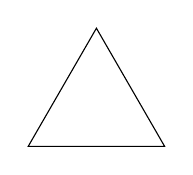
\begin{tikzpicture}
\draw (90:1) -- (90+120:1) -- (90-120:1) -- cycle;
\end{tikzpicture}
\end{exampleblock}

\end{frame}





\begin{frame}
\frametitle{Retângulos}

\begin{block}{Retângulo}\ttfamily
\purple{\string\draw} ... \texttt{\green{\textit{ponto-inicial}} \blue{rectangle} \green{\textit{ponto-final}};}
\end{block}

\bigskip 

\begin{code*}
\string\draw\ \green{(0,0)} \blue{rectangle} \green{(2,1)}  \blue{rectangle} \green{(3,3)};

\bigskip\centering

\tikz{\draw (0,0) rectangle (2,1) rectangle (3,3);} 
\end{code*}

\end{frame}









\begin{frame}
  \frametitle{Círculos}

  \begin{block}{Círculos (centro no ponto atual)}\ttfamily
    \purple{\string\draw} ... \blue{\textit{ponto-centro}} \green{\texttt{circle (\textit{raio})};}
  \end{block}

\bigskip

\begin{multicols}{2}

\begin{code*}\footnotesize
\string\begin\ac{}tikzpicture\fc{}\\
\mbox{}\ \ \string\draw[thick]\ (0,0) \purple{circle\ (1)};\\
\mbox{}\ \ \string\draw\ (0,0)\ --\\
\mbox{}\ \ \ \ \ \gray{\textit{\pc{} escrevendo no meio do segmento}}\\
\mbox{}\ \ \ \ \ \green{node[right]\ \ac{}\dolar{}r=1\dolar{}\fc{}}\\
\mbox{}\ \ \ \ (0,1);\\
\string\end\ac{}tikzpicture\fc{}
\end{code*}

\mbox{}\hfill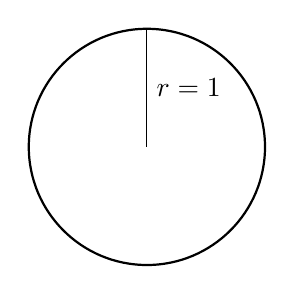
\begin{tikzpicture}[scale=1.5]
  \draw[thick] (0,0) circle (1);
  \draw (0,0) -- node[pos=.5,right] {$r=1$} (0,1);
\end{tikzpicture}

\end{multicols}

% \bigskip

% \begin{multicols}{2}

% \begin{code*}\scriptsize
% \string\begin\ac{}tikzpicture\fc{}\\
% \string\draw[thick]\ +(1,0)\ --\ +(0,1)\ --\ +(-1,0)\ --\ +(0,-1)\ --\ cycle;\\
% \string\fill\ circle\ (.1);\\
% \string\end\ac{}tikzpicture\fc{}
% \end{code*}

% \ \\\hfill \begin{tikzpicture}[scale=.5]
% \draw[thick] +(1,0) -- +(0,1) -- +(-1,0) -- +(0,-1) -- cycle;
% \fill circle (.1);
% \end{tikzpicture}


%\end{multicols}


\end{frame}

\begin{frame}
  \frametitle{Arcos de circunferência}
  \begin{block}{Arcos}
    \texttt{\purple{\string\draw} ... \red{\textit{ponto-inicial}}\\
      \mbox{}\ \ \ \ \ \ \blue{arc} (\green{\textit{ângulo-inicial}}:\blue{\textit{ângulo-final}}:\purple{\textit{raio}})}\bigskip

    O arco \blue{inicia no ponto atual.}\medskip

    Isto é ideal para colar
    vários arcos para uma curva suave.
  \end{block}

\bigskip

  \begin{alertblock}{Parece antinatural}
    \red{O ponto atual não é o centro}, como costuma-se pensar no início.
  \end{alertblock}

\end{frame}

\begin{frame}
  \frametitle{Exemplo com \texttt{arc}}

  \begin{exampleblock}{Ângulos opostos pelo vértice}
    \medskip

%    \begin{minipage}{.9\linewidth}
\scriptsize\ttfamily
    \purple{\string\begin\ac{}tikzpicture\fc}\\
    \mbox{}\ \ \string\draw\ (-1,0)\ --\ (2,0);\ \ \ \ \ \ \ \ \ \ \ \ \ \ \ \ \ \ \ \gray{\textit{\pc{}\ reta\ inferior}}\\
    \mbox{}\ \ \string\draw\ (-1,0\ |-\ 50:1)\ --\ (2,0\ |-\ 50:1);\ \ \ \gray{\textit{\pc{}\ paralela\ superior}}\\
    \mbox{}\ \ \string\draw\ (50:-.7)\ --\ (50:1.7);\ \ \ \ \ \ \ \ \ \ \ \ \ \ \gray{\textit{\pc{}\ transversal}}\\
    \mbox{}\ \ \string\draw\ (0:.3)\ \blue{arc\ (0:50:.3)};\ \ \ \ \ \ \ \ \ \ \ \ \ \ \gray{\textit{\pc{}\ arco\ inferior}}\\
    \mbox{}\ \ \string\draw\ (25:.25)\ --\ (25:.35);\ \ \ \ \ \ \ \ \ \ \ \ \ \ \gray{\textit{\pc{}\ marquinha\ inferior}}\\
    \mbox{}\ \ \gray{\textit{\pc{}\ usando\ coordenadas\ relativas\ agora}}\\
    \mbox{}\ \ \string\draw\ (50:1)\ ++(0:-.3)\ \blue{arc\ (0:50:-.3)};\ \ \ \gray{\textit{\pc{}\ arco\ superior}}\\
    \mbox{}\ \ \string\draw\ (50:1)\ ++(25:-.25)\ --\ ++(25:-.1);\ \ \gray{\textit{\pc{}\ marquinha\ superior}}\\
    \purple{\string\end\ac{}tikzpicture\fc}
%\end{minipage}

    \centering
    \begin{tikzpicture}
      \draw (-1,0) -- (2,0);                  % reta inferior
      \draw (-1,0 |- 50:1) -- (2,0 |- 50:1);  % paralela superior
      \draw (50:-.7) -- (50:1.7);             % transversal
      \draw (0:.3) arc (0:50:.3);             % arco inferior
      \draw (25:.25) -- (25:.35);             % marquinha inferior
      % usando coordenadas relativas agora
      \draw (50:1) ++(0:-.3) arc (0:50:-.3);  % arco superior
      \draw (50:1) ++(25:-.25) -- ++(25:-.1); % marquinha superior
    \end{tikzpicture}
  \end{exampleblock}

\end{frame}


\begin{frame}
  \frametitle{Exercício com \texttt{arc}: logotipo da SBM}

  \begin{itemize}
  \item Logotipo da Sociedade Brasileira de Matemática: espiral de Euclides.
    
    \begin{center}
      \imagem[width=3cm]{sbm.png}
    \end{center}

  \item A espiral: construída com quartos de circunferência no
    retângulo áureo: os lados dos quadrados estão na proporção áurea
    \[
    \varphi= \frac{1+\sqrt5}{2} \implies \frac{1}{\varphi}=\frac{\sqrt5-1}{2}
    \]

  \item De um quadrado para outro, divide-se por $\varphi$.
  \end{itemize}
\end{frame}

\begin{frame}
  \frametitle{Proposta de resolução preto e branco}
  
  \begin{itemize}
  \item calculamos os pontos no final dos arcos, \\
    nomeando-os com
    \texttt{\green{coordinate (p\textit{\blue{n}})}}, até $p_4$
  \item depois, traçamos os retângulos com cantos $p_{n-1}$ e $p_n$
  \item note que podemos \purple{fazer contas no código! \smiley}
  \end{itemize}

  \bigskip

  \newsavebox{\codebox}
  \savebox{\codebox}{\parbox{.73\textwidth}{%
      \ttfamily\footnotesize
    \purple{\string\begin\ac{}tikzpicture\fc{}}\\
      \gray{\textit{\pc{}\ definimos\ \string\iphi\ =\ 1/phi}}\\
      \brown{\string\newcommand\ac\string\iphi\fc\ac{}0.618\fc}\\
      \string\draw\ (0,0)\ \green{coordinate\ (p0)}\\
      \mbox{}\ \  \blue{arc(180\ :\ \ \ 90\ :\ 1\ \ \ \ \ \ )}\ \green{coordinate\ (p1)}\\
      \mbox{}\ \  \blue{arc( 90\ :\ \ \ \ 0\ :\ \string\iphi\ \ )}\
      \green{coordinate\ (p2)}\\
      \mbox{}\ \  \blue{arc( \ 0\ :\ \ -90\ :\ \string\iphi\textasciicircum{}2)}\ \green{coordinate\ (p3)}\\
      \mbox{}\ \  \blue{arc(-90\ :\ -180\ :\ \string\iphi\textasciicircum{}3)}\ \green{coordinate\ (p4)};\\
      \string\draw\ (p0)\ rectangle\ (p1)\ rectangle\ (p2)\ \\
      \mbox{}\ \ \ \ \ \ \ \ \ \ \ rectangle\ (p3)\ rectangle\ (p4);\\
      \purple{\string\end\ac{}tikzpicture\fc{}}}}

  \begin{tabular}{l@{}l}
    \usebox{\codebox}
    &
    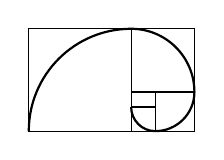
\begin{tikzpicture}[scale=1.3]
      \def\iphi{0.618} % definimos \iphi = 1/phi
      \draw[thick] (0,0) coordinate (p0)
          arc(180 : 90 : 1) coordinate (p1)
          arc(90 : 0 : \iphi) coordinate (p2)
          arc(0 : -90 : \iphi^2) coordinate (p3)
          arc(-90 : -180 : \iphi^3) coordinate (p4);
      \draw (p0) rectangle (p1) rectangle (p2) 
                 rectangle (p3) rectangle (p4);
  \end{tikzpicture}
\end{tabular}
 
\end{frame}

\begin{frame}
  \frametitle{Resolução colorida (segredo \smiley)}

  \centering
    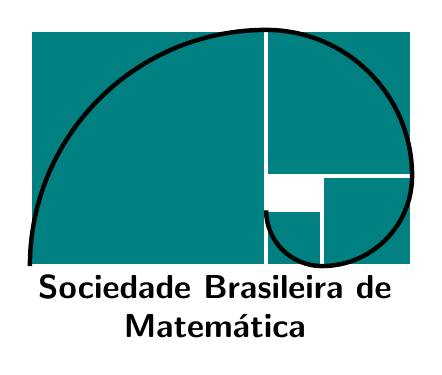
\begin{tikzpicture}[scale=3]
      \def\iphi{0.618} % definimos \iphi = 1/phi
      \draw[very thin] (0,0) coordinate (p0)
          arc(180 : 90 : 1) coordinate (p1)
          arc(90 : 0 : \iphi) coordinate (p2)
          arc(0 : -90 : \iphi^2) coordinate (p3)
          arc(-90 : -180 : \iphi^3) coordinate (p4);
      \draw[very thick,white,fill=teal] (p0) rectangle (p1) rectangle (p2) 
                 rectangle (p3) rectangle (p4);
      \draw[ultra thick] (0,0) arc(180 : 90 : 1) arc(90 : 0 : \iphi) 
          arc(0 : -90 : \iphi^2) arc(-90 : -180 : \iphi^3);
      \node[below right,xshift=-0.7] at (p0) {\parbox{4.5cm}{\centering\large\bfseries\textsf{Sociedade Brasileira de Matemática}}};
  \end{tikzpicture}
  

\end{frame}

\begin{frame}
  \frametitle{Linhas curvas}
  \begin{block}{Linhas curvas}
    ligue pontos com comando\\
    \texttt{\blue{to [out=}\green{\textit{âng-saída}}\blue{,in=}\green{\textit{âng-chegada}}\blue{]}}
  \end{block}

\bigskip

\begin{code*}
\string\draw[->]\ (0,0)\ to\ [out=90,in=270]\ (1,1);
\ \ \begin{tikzpicture}
  \draw[->] (0,0) to [out=90,in=270] (1,1);
\end{tikzpicture}
\end{code*}

\end{frame}

\begin{frame}
  \frametitle{Bèziers}
  
  \begin{block}{Bèziers}
    1 ponto de controle: \texttt{\blue{..\ controls} \green{\textit{ponto}} \blue{..}}\\
    2 pontos de controle: \texttt{\blue{..\ controls}
        \green{\textit{ponto1}} \red{and} \green{\textit{ponto2}} \blue{..}}\\
  \end{block}
  

\bigskip

\begin{code*}\footnotesize
\string\draw[thick] \ (-1,0) \blue{..\ controls (0,1) ..}\ (1,0);\\
\string\draw[thick] \ (2,0) \blue{.. controls (2,1) and (4,1) ..} (4,0);\\
\gray{\textit{\pc\ linhas para ver os controles...}}\\
\string\draw[dotted] (-1,0) -- (0,1) -- (1,0);\\
\string\draw[dotted] (2,0) -- (2,1) -- (4,1) -- (4,0);


\bigskip
\centering
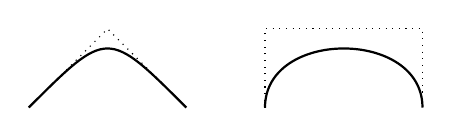
\begin{tikzpicture}
  \draw[thick] (-1,0) .. controls (0,1) .. (1,0);
  \draw[thick] (2,0) .. controls (2,1) and (4,1) .. (4,0);
  \draw[dotted] (2,0) -- (2,1) -- (4,1) -- (4,0);
  \draw[dotted] (-1,0) -- (0,1) -- (1,0);
\end{tikzpicture}
\end{code*}


\end{frame}

\section{Estilos de linha}

\begin{frame}
  \frametitle{Alterando estilos de linhas}
  \begin{block}{Estilos de linha}
    Coloque os estilos de linha no \green{parâmetro opcional} do
    \blue{\texttt{\bs draw}},\\
    separados por vírgula se tiver mais de um.
  \end{block}

\bigskip

\begin{code*}\small
\ \ \blue{\string\draw}\brown{[<->,very thick,dashed,blue]}\ (0,0)\ --\ (2,0);
\bigskip

\centering
  \tikz \draw[<->,very thick,dashed,blue] (0,0) -- (2,0);
\end{code*}

\end{frame}

\begin{frame}
  \frametitle{Setas}
  \begin{block}{Setas}
    \begin{itemize}
    \item[\texttt{->}] seta normal \tikz \draw[->] (0,0)--(1,0);
    \item[\texttt{<->}] seta com ponta dos dois lados \tikz \draw[<->] (0,0)--(1,0);
    \item[\texttt{|->}] seta ``maps to''
	\tikz \draw[|->] (0,0)--(1,0);

    \end{itemize}
  \end{block}
\end{frame}

\begin{frame}
  \frametitle{Grossura da linha}

  \begin{block}{Grossura}

    \begin{description}
      \item[ultra thin] finíssima \tikz \draw[ultra thin] (0,0)--(1,0);
      \item[very thin] muito fina \tikz \draw[very thin] (0,0)--(1,0);
      \item[thin] fina \tikz \draw[thin] (0,0)--(1,0);
      \item[thick] “grossinha” \tikz \draw[thick] (0,0)--(1,0);
      \item[very thick] grossa \tikz \draw[very thick] (0,0)--(1,0);
      \item[ultra thick] bem grossa \tikz \draw[ultra thick] (0,0)--(1,0);
      \item[semithick] = normal \tikz \draw (0,0)--(1,0);
    \end{description}

  \end{block}
\end{frame}

\begin{frame}
  \frametitle{Tracejado e pontilhado}

  \begin{block}{Tracejado e pontilhado}
    Os principais estilos são \blue{dashed} (tracejado) e
    \blue{dotted}
    (pontilhado)\\
    Podem ser mais espassados (\green{\texttt{loosely ...}}) ou
    condensados \green{\texttt{densely ...}}.


  \begin{description}
  \item[dashed] \tikz \draw[dashed] (0,0) -- (1,0);
  \item[loosely dashed] \tikz \draw[loosely dashed] (0,0) -- (1,0);
  \item[densely dashed] \tikz \draw[densely dashed] (0,0) -- (1,0);
  \item[dotted] \tikz \draw[dotted] (0,0) -- (1,0);
  \item[loosely dotted] \tikz \draw[loosely dotted] (0,0) -- (1,0);
  \item[densely dotted] \tikz \draw[densely dotted] (0,0) -- (1,0);
  \end{description}
  \end{block}

\end{frame}

\section{Escrevendo nomes}

\begin{frame}
  \frametitle{Escrevendo nomes: \texttt{\string\node}}

  \begin{block}{Comando node}
    \ttfamily
    \purple{\string\node}\brown{[opt]} \blue{at \textit{ponto}} 
    \green{\ac \textit{texto}\fc}
  \end{block}

  \begin{block}{Opções}
    \begin{itemize}\ttfamily
    \item above, below, left, right,
    \item above right, below left, etc,
    \item xshift = \textit{comprimento}
    \item yshift = \textit{comprimento}
    \end{itemize}
  \end{block}
\end{frame}

\begin{frame}
  \frametitle{Exemplo de \texttt{\string\node}}


\begin{block}{Comando node}
    \ttfamily
    \purple{\string\node}\brown{[opt]} \blue{at \textit{ponto}} 
    \green{\ac \textit{texto}\fc}
  \end{block}

  \begin{exampleblock}{}\ttfamily
    \string\begin\ac{}tikzpicture\fc{}\\
    \ \ \string\draw[fill=red]\ (0,0)\ coordinate\ (A)\ circle\ (2pt);\\
    \ \ \purple{\string\node[above\ right]\ at\ (A)\ \ac{}\dolar{}A\dolar{}\fc{};}\\
    \string\end\ac{}tikzpicture\fc{}

\centering
    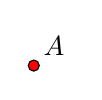
\begin{tikzpicture}
      \draw[fill=red] (0,0) coordinate (A) circle (2pt);
      \node[above right] at (A) {$A$};
    \end{tikzpicture}

  \end{exampleblock}
\end{frame}

\begin{frame}
  \frametitle{Nomeando caminhos}

  \begin{block}{\texttt{node} no meio de comandos \texttt{\string\draw}}
    \ttfamily \green{\string\draw} ... \purple{node}\brown{[opts]} \blue{\ac\textit{texto}\fc}\ ...;
  \end{block}

  \begin{block}{Opções}
    \begin{itemize}\ttfamily
    \item pos=\textit{número entre 0 e 1} (para caminhos)
    \item right, above, etc.
    \item xshift=\textit{comprimento}
    \item yshift=\textit{comprimento}
    \end{itemize}
  \end{block}
\end{frame}

\begin{frame}
  \frametitle{Exemplo de node no meio do caminho}
  \begin{exampleblock}{}
    \ttfamily
    \string\begin\ac{}tikzpicture\fc{}\\
    \ \ \string\draw\ (0,0)\ --\ node[pos=.3,below]\ \ac{}\dolar{}a\dolar{}\fc{}\ \\
    \ \ \ \ \ \ \ \ (2,0)\ to[out=90,in=0]\ node[pos=.6]\ \ac{}\dolar{}b\dolar{}\fc{}\\
    \ \ \ \ \ \ \ \ (1.5,1);\ \ \\
    \string\end\ac{}tikzpicture\fc{}

\bigskip
    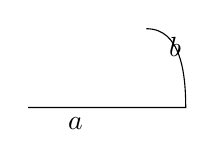
\begin{tikzpicture}
      \draw (0,0) -- node[pos=.3,below] {$a$} 
            (2,0) to[out=90,in=0] node[pos=.6] {$b$}
            (1.5,1);  
    \end{tikzpicture}
  \end{exampleblock}
\end{frame}


\section{Plotando}

\begin{frame}
  \frametitle{Plotando curvas}

  \begin{block}{Plotando}
    \texttt{\string\draw[\textit{opções}] plot
      (\ac\textit{fórmula-x}\fc\red{,}\ac\textit{fórmula-y}\fc)}

\mbox{}\qquad ou

    \texttt{\string\draw[\textit{opções}] plot (\ac\textit{fórmula-âng}\fc\red{:}\ac\textit{fórmula-raio}\fc)}


\texttt{variable=\string\var,domain=inicio:fim,smooth,samples=num}
  \end{block}

\begin{code*}\scriptsize    
\string\begin\ac{}tikzpicture\fc{}\\
\ \ \string\draw[->]\ (-3,0)\ --\ (4.2,0)\ node[right]\ \ac{}\dolar{}x\dolar{}\fc{};\\
\ \ \string\draw[->]\ (0,-3)\ --\ (0,4.2)\ node[above]\ \ac{}\dolar{}y\dolar{}\fc{};\\
\ \ \string\draw[scale=0.5,domain=-3:3,smooth,variable=\string\x,blue]\\ plot\ (\ac{}\string\x\fc{},\ac{}\string\x*\string\x\fc{});\\
\ \ \string\draw[scale=0.5,domain=-3:3,smooth,variable=\string\y,red]\\ plot\ (\ac{}\string\y*\string\y\fc{},\ac{}\string\y\fc{});\\
\string\end\ac{}tikzpicture\fc{}
\end{code*}

\centering
\begin{tikzpicture}[scale=.5]
  \draw[->] (-3,0) -- (4.2,0) node[right] {$x$};
  \draw[->] (0,-3) -- (0,4.2) node[above] {$y$};
  \draw[scale=0.5,domain=-3:3,smooth,variable=\x,blue] plot ({\x},{\x*\x});
  \draw[scale=0.5,domain=-3:3,smooth,variable=\y,red]  plot ({\y*\y},{\y});
\end{tikzpicture}
    

%  \end{exampleblock}
\end{frame}


\begin{frame}
  \frametitle{Cores}

\begin{multicols}{3}
red \tikz \fill[red] (0,0) rectangle (1,0.4);

blue \tikz \fill[blue] (0,0) rectangle (1,0.4);

green \tikz \fill[green] (0,0) rectangle (1,0.4);

black \tikz \fill[black] (0,0) rectangle (1,0.4);

yellow \tikz \fill[yellow] (0,0) rectangle (1,0.4);

white \tikz \draw (0,0) rectangle (1,0.4);

cyan \tikz \fill[cyan] (0,0) rectangle (1,0.4);

magenta \tikz \fill[magenta] (0,0) rectangle (1,0.4);

gray \tikz \fill[gray] (0,0) rectangle (1,0.4);

darkgray \tikz \fill[darkgray] (0,0) rectangle (1,0.4);

lightgray \tikz \fill[lightgray] (0,0) rectangle (1,0.4);

brown \tikz \fill[brown] (0,0) rectangle (1,0.4);

lime \tikz \fill[lime] (0,0) rectangle (1,0.4);

olive \tikz \fill[olive] (0,0) rectangle (1,0.4);

orange \tikz \fill[orange] (0,0) rectangle (1,0.4);

pink \tikz \fill[pink] (0,0) rectangle (1,0.4);

purple \tikz \fill[purple] (0,0) rectangle (1,0.4);

teal \tikz \fill[teal] (0,0) rectangle (1,0.4);

violet \tikz \fill[violet] (0,0) rectangle (1,0.4);

\end{multicols}


\end{frame}


\endinput
\part{Figuras com \Tikz}

\begin{frame}
  \frametitle{\Tikz}
  
  \begin{itemize}
  \item O \Tikz\ é uma linguagem que gera figuras, a partir de uma
    descrição da mesma em termos de linhas, formas e texto.
  \item gráficos são vetoriais e de alta qualidade
  \item já são parte do documento \tikz \draw[color=blue,thick] (0,0)
    circle (.7ex); sendo \tikz \draw[rotate=20,purple,thick] (0,0) rectangle
    (1ex,.6ex); fáceis 
    \tikz \draw[thick,green!50!black] (0,0) -- (1ex,0) -- (60:1ex) --cycle;
    de misturar.
  \end{itemize}
 
\end{frame}

\begin{frame}
  \frametitle{Figuras com \Tikz}

  \begin{itemize}
  \item Usar pacote \green{\texttt{tikz}} no preâmbulo
  \item Usar ambiente \blue{\texttt{tikzpicture}}
  \item Dentro do ambiente, usar comandos\\
    \purple{\texttt{\bs draw}} --- para traçar linhas\\
    \purple{\texttt{\bs fill}} --- para áreas preenchidas\\
    que terminam com ponto-e-vírgula \texttt{;}
  \item tem \green{parâmetros opcionais} para alterar estilos
    de linha e preenchimento

\begin{multicols}{2}
\begin{code*}\footnotesize
\string\begin\ac{}tikzpicture\fc{}\\
\string\draw[->,blue]\ \ (0,1)\ --\ (1,0);\\
\string\end\ac{}tikzpicture\fc{}
\end{code*}

\begin{tikzpicture}
\draw[->,blue]  (0,1) -- (1,0);
\end{tikzpicture}
\end{multicols}

  \end{itemize}
\end{frame}

\section{Caminhos}

\begin{frame}
  \frametitle{Tipos de caminhos}

  \begin{block}{Tipos de caminhos}
    \begin{itemize}
    \item segmentos
    \item círculos
    \item arcos de circunferência
    \item linhas especificando ângulos de saída e chegada
    \item béziers
    \end{itemize}
  \end{block}

\bigskip

  Caminhos podem ser
  \begin{itemize}
  \item abertos
  \item fechados (termina com \texttt{-{}- cycle})
  \end{itemize}

\end{frame}

\begin{frame}
  \frametitle{Pontos}

  \begin{block}{Pontos}
    Dois valores entre parênteses.
  \end{block}
\bigskip

  Podem ser em \green{coordenadas}
  \begin{description}
  \item[cartesianas] valores $(x,y)$ separados por vírgula --- \texttt{(0,1)}
  \item[polares] valores $(\theta:r)$ separados por 2-pontos --- \texttt{(30:1)}
  \end{description}
\end{frame}

\begin{frame}
  \frametitle{Coordenadas em valor absoluto ou relativo}

  \begin{block}{Tipos de coordanadas}
    \begin{description}
    \item[absoluto] Determina o ponto\\
      \blue{\texttt{(1,0)}} --- ponto de coordenadas $(1,0)$.
    \item[relativo] Adiciona à posição atual: comece ponto com
      \green{\texttt{++}}
      \blue{\texttt{++(1,0)}} --- se o ponto anterior era $(2,2)$, vai
      para o ponto $(3,2)$.

    \item[relativo sem atualização] Adiciona à posição atual\\
      mas \red{não atualiza posição}:\\ comece ponto com \green{\texttt{+}}.

      Exemplo: \blue{\texttt{+(1,0)}} --- se o ponto anterior era
      $(2,2)$, denota o ponto $(3,2)$, mas ponto atual fica em
      $(2,2)$.
    \end{description}
  \end{block}

\end{frame}

\begin{frame}
  \frametitle{Segmentos}

  \begin{block}{Segmentos}
    Sequência de pontos ligados por \texttt{--}.
  \end{block}

\begin{multicols}{2}
\begin{code*}
\string\begin\ac{}tikzpicture\fc{}\\
\ \ \string\draw[->]\ (0,0)\ --\ (30:1)\ --\ ++(1,0)\ --\ ++(0,1);\\
\string\end\ac{}tikzpicture\fc{}
\end{code*}

\begin{tikzpicture}
\draw[->] (0,0) -- (30:1) -- ++(1,0) -- ++(0,1);
\end{tikzpicture}
\end{multicols}

\end{frame}





\begin{frame}
\frametitle{Retângulos}

\begin{block}{}
Comando \texttt{\green{ponto-inicial} \blue{rectangle} \green{ponto final}}
\end{block}

\bigskip 

\begin{code*}
\string\draw\ (0,0) rectangle (2,1);
\ \ 
\tikz{\draw (0,0) rectangle (2,1);} 
\end{code*}

\end{frame}

\begin{frame}
  \frametitle{Círculos}
  \begin{block}{Círculos (centro no ponto atual)}
    \green{\texttt{circle (\textit{raio})}}
  \end{block}

\bigskip

\begin{multicols}{2}

\begin{code*}
\string\begin\ac{}tikzpicture\fc{}[scale=.5]\\
\ \ \string\draw\ circle\ (1);\\
\ \ \string\draw\ (0,0)\ --\ (0,1);\\
\string\end\ac{}tikzpicture\fc{}
\end{code*}

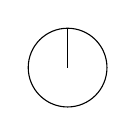
\begin{tikzpicture}[scale=.5]
  \draw circle (1);
  \draw (0,0) -- (0,1);
\end{tikzpicture}
\end{multicols}

\bigskip
\begin{multicols}{2}
\begin{code*}\scriptsize
\string\begin\ac{}tikzpicture\fc{}\\
\string\draw[thick]\ +(1,0)\ --\ +(0,1)\ --\ +(-1,0)\ --\ +(0,-1)\ --\ cycle;\\
\string\fill\ circle\ (.1);\\
\string\end\ac{}tikzpicture\fc{}
\end{code*}

\ \\\hfill 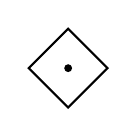
\begin{tikzpicture}[scale=.5]
\draw[thick] +(1,0) -- +(0,1) -- +(-1,0) -- +(0,-1) -- cycle;
\fill circle (.1);
\end{tikzpicture}


\end{multicols}

\end{frame}

\begin{frame}
  \frametitle{Arcos de circunferência}
  \begin{block}{Arcos}
    Especificar \green{ângulo inicial}, \blue{ângulo final} e
    \purple{raio}.\\
    O arco \blue{inicia} no ponto atual.
  \end{block}

  \begin{alertblock}{}
    O ponto atual \red{não} é o centro, como costuma-se pensar no início.
  \end{alertblock}

\bigskip

\begin{code*}
\ \ \string\draw\ (0:1)--(0,0)\ --\ (30:1)\ \ arc\ (30:60:1);
\ \ 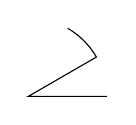
\begin{tikzpicture}
  \draw (0:1)--(0,0) -- (30:1)  arc (30:60:1);
\end{tikzpicture}
\end{code*}

\end{frame}

\begin{frame}
  \frametitle{Linhas curvas}
  \begin{block}{Linhas curvas}
    ligue pontos com comando
    \texttt{\blue{to [out=}\green{\textit{âng-saída}}\blue{,in=}\green{\textit{âng-chegada}}\blue{]}}
  \end{block}

\bigskip

\begin{code*}
\string\draw[->]\ (0,0)\ to\ [out=90,in=270]\ (1,1);
\ \ \begin{tikzpicture}
  \draw[->] (0,0) to [out=90,in=270] (1,1);
\end{tikzpicture}
\end{code*}

\end{frame}

\section{Estilos de linha}

\begin{frame}
  \frametitle{Alterando estilos de linhas}
  \begin{block}{Estilos de linha}
    Coloque os estilos de linha no \green{parâmetro opcional} do
    \blue{\texttt{\bs draw}},\\
    separados por vírgula se tiver mais de um.
  \end{block}

\bigskip

\begin{code*}
\ \ \string\draw[->,thick]\ (0,0)\ --\ (1,0);
  \tikz \draw[->,thick] (0,0) -- (1,0);
\end{code*}

\end{frame}

\begin{frame}
  \frametitle{Setas}
  \begin{block}{Setas}
    \begin{itemize}
    \item[\texttt{->}] seta normal \tikz \draw[->] (0,0)--(1,0);
    \item[\texttt{<->}] seta com ponta dos dois lados \tikz \draw[<->] (0,0)--(1,0);
    \end{itemize}
  \end{block}
\end{frame}

\begin{frame}
  \frametitle{Grossura da linha}

  \begin{block}{Grossura}

    \begin{description}
      \item[ultra thin] finíssima \tikz \draw[ultra thin] (0,0)--(1,0);
      \item[very thin] muito fina \tikz \draw[very thin] (0,0)--(1,0);
      \item[thin] fina \tikz \draw[thin] (0,0)--(1,0);
      \item[thick] “grossinha” \tikz \draw[thick] (0,0)--(1,0);
      \item[very thick] grossa \tikz \draw[very thick] (0,0)--(1,0);
      \item[ultra thick] bem grossa \tikz \draw[ultra thick] (0,0)--(1,0);
      \item[semithick] = normal \tikz \draw (0,0)--(1,0);
    \end{description}

  \end{block}
\end{frame}

\begin{frame}
  \frametitle{Tracejado e pontilhado}

  \begin{block}{Tracejado e pontilhado}
    Os principais estilos são \blue{dashed} (tracejado) e
    \blue{dotted}
    (pontilhado)\\
    Podem ser mais espassados (\green{\texttt{loosely ...}}) ou
    condensados \green{\texttt{densely ...}}.


  \begin{description}
  \item[dashed] \tikz \draw[dashed] (0,0) -- (1,0);
  \item[loosely dashed] \tikz \draw[loosely dashed] (0,0) -- (1,0);
  \item[densely dashed] \tikz \draw[densely dashed] (0,0) -- (1,0);
  \item[dotted] \tikz \draw[dotted] (0,0) -- (1,0);
  \item[loosely dotted] \tikz \draw[loosely dotted] (0,0) -- (1,0);
  \item[densely dotted] \tikz \draw[densely dotted] (0,0) -- (1,0);
  \end{description}
  \end{block}

\end{frame}

\begin{frame}
  \frametitle{Cores}

\begin{multicols}{3}
red \tikz \fill[red] (0,0) rectangle (1,0.4);

blue \tikz \fill[blue] (0,0) rectangle (1,0.4);

green \tikz \fill[green] (0,0) rectangle (1,0.4);

black \tikz \fill[black] (0,0) rectangle (1,0.4);

yellow \tikz \fill[yellow] (0,0) rectangle (1,0.4);

white \tikz \draw (0,0) rectangle (1,0.4);

cyan \tikz \fill[cyan] (0,0) rectangle (1,0.4);

magenta \tikz \fill[magenta] (0,0) rectangle (1,0.4);

gray \tikz \fill[gray] (0,0) rectangle (1,0.4);

darkgray \tikz \fill[darkgray] (0,0) rectangle (1,0.4);

lightgray \tikz \fill[lightgray] (0,0) rectangle (1,0.4);

brown \tikz \fill[brown] (0,0) rectangle (1,0.4);

lime \tikz \fill[lime] (0,0) rectangle (1,0.4);

olive \tikz \fill[olive] (0,0) rectangle (1,0.4);

orange \tikz \fill[orange] (0,0) rectangle (1,0.4);

pink \tikz \fill[pink] (0,0) rectangle (1,0.4);

purple \tikz \fill[purple] (0,0) rectangle (1,0.4);

teal \tikz \fill[teal] (0,0) rectangle (1,0.4);

violet \tikz \fill[violet] (0,0) rectangle (1,0.4);

\end{multicols}

\end{frame}


%%% Local Variables: 
%%% mode: latex
%%% TeX-master: "../latex-curto"
%%% End: 
